\documentclass[10pt, landscape]{article}
\usepackage[scaled=0.92]{helvet}
\usepackage{calc}
\usepackage{multicol}
\usepackage[a4paper,margin=3mm,landscape]{geometry}
\usepackage{amsmath,amsthm,amsfonts,amssymb}
\usepackage{color,graphicx,overpic}
\usepackage{hyperref}
\usepackage{newtxtext} 
\usepackage{enumitem}
\usepackage[table]{xcolor}
\usepackage{mathtools}
\setlist{nosep}
% for including images
\graphicspath{ {../images/} }

\pdfinfo{
  /Title (CS4221.pdf)
  /Creator (TeX)
  /Producer (pdfTeX 1.40.0)
  /Author (Gavin Chiam)
  /Subject (CS4221 Midterm Cheatsheet)
/Keywords (CS4221, nus, cheatsheet, pdf)}

% Turn off header and footer
\pagestyle{empty}

% redefine section commands to use less space
\makeatletter
\renewcommand{\section}{\@startsection{section}{1}{0mm}%
  {-1ex plus -.5ex minus -.2ex}%
  {0.5ex plus .2ex}%x
{\normalfont\large\bfseries}}
\renewcommand{\subsection}{\@startsection{subsection}{2}{0mm}%
  {-1explus -.5ex minus -.2ex}%
  {0.5ex plus .2ex}%
{\normalfont\normalsize\bfseries}}
\renewcommand{\subsubsection}{\@startsection{subsubsection}{3}{0mm}%
  {-1ex plus -.5ex minus -.2ex}%
  {1ex plus .2ex}%
{\normalfont\small\bfseries}}%
\makeatother

\renewcommand{\familydefault}{\sfdefault}
\renewcommand\rmdefault{\sfdefault}
%  makes nested numbering (e.g. 1.1.1, 1.1.2, etc)
\renewcommand{\labelenumii}{\theenumii}
\renewcommand{\theenumii}{\theenumi.\arabic{enumii}.}
\renewcommand\labelitemii{•}
\renewcommand\labelitemiii{•}

\definecolor{mathblue}{cmyk}{1,.72,0,.38}
\everymath\expandafter{\the\everymath \color{mathblue}}

% Don't print section numbers
\setcounter{secnumdepth}{0}

\setlength{\parindent}{0pt}
\setlength{\parskip}{0pt plus 0.5ex}
%% adjust spacing for all itemize/enumerate
\setlength{\leftmargini}{0.5cm}
\setlength{\leftmarginii}{0.5cm}
\setlist[itemize,1]{leftmargin=2mm,labelindent=1mm,labelsep=1mm}
\setlist[itemize,2]{leftmargin=4mm,labelindent=1mm,labelsep=1mm}
\setlist[itemize,3]{leftmargin=4mm,labelindent=1mm,labelsep=1mm}

% adding my commands
\input{../../commands/style-helpers.tex}

% -----------------------------------------------------------------------

\begin{document}
\raggedright
\footnotesize
\begin{multicols*}{4}
  % multicol parameters
  \setlength{\columnseprule}{0.25pt}

  \begin{center}
    \fbox{%
      \parbox{0.8\linewidth}{\centering \textcolor{black}{
          {\Large\textbf{CS4221}}
        \\ \normalsize{AY25/26 SEM 2}}
        \\ {\footnotesize \textcolor{gray}{github/Gavino3o}}
      }%
    }
  \end{center}

  \section{Entity Relationship Diagrams}
  \begin{itemize}
    \item Entity-relationship model is value-oriented. Values are atomic data types (INTEGER, TEXT, etc).
    \item Entity sets: rectangles, with name in plural noun form.
    \item Attributes: circles, with name in singular noun form.
    \item Derived attributes: dashed line connected to a circle. (May be derived from other attributes, or from other entity sets.)
    \item Relationship sets: diamonds, with name in verb form. Connected to entity sets with lines.
    \item \textbf{No duplicates} for entity and relationship sets
    \item Relationships can have attributes. However, \textbf{relationships are not distinguished by their attributes}, but by the entities they connect. \textbf{No black circle!} (e.g cannot have customer downloading same game multiple times on different devices)
    \item\textbf{n-ary relationships:} relationship sets that connect more than 2 entity sets. All entities must be participating; no entity can be missing.
    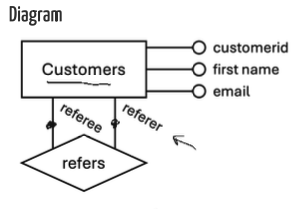
\includegraphics[width=0.85\linewidth, height = 100px]{er2.png} 
    \item \textbf{Attribute Promotion}: Converting an attribute of a relationship set into an entity set. This is done when the attribute has multiple values for the same relationship (e.g. a customer can download the same game on multiple devices, so we promote the "device" attribute into an entity set).
    \item \textbf{Aggregate}: A relationship set can be treated as an entity set when it participates in another relationship set. This is done by enclosing the relationship set in a rectangle, and connecting it to the new relationship set with a line.
    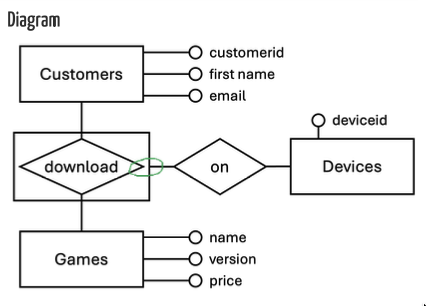
\includegraphics[width=0.85\linewidth, height = 100px]{er3.png} 
    \item \textbf{Identifying Attributes}: One or more UNIQUE NOT NULL attributes that can be used to identify an entity. Black Circle.
    \item Entity set can have multiple candidate keys, but only one primary key. 
    \item \textbf{Partial Identification}: When an entity cannot be identified by its own attributes alone, but can be identified by a combination of its own attributes and the identifying attributes of another entity set. Connect the partial identifier (attribute) to the participation of dominant entity.
    \item Can have multiple dominant entity sets. Also can have other (non-partial) key.
    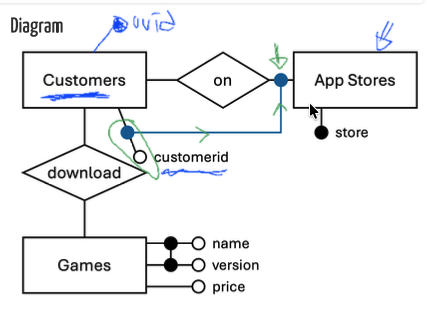
\includegraphics[width=0.85\linewidth, height = 100px]{er4.png} 
    \item \textbf{Participation Constraints}: Between entity and relationship set. Restricted by (minimum, maximum) cardinality.
    \textbf{Default: (0, n)}
    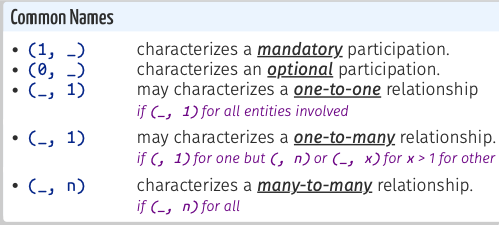
\includegraphics[width=0.97\linewidth]{participation_constraint.png}
    \item Weak entities can only be defined for a (1, 1) constraint. 
    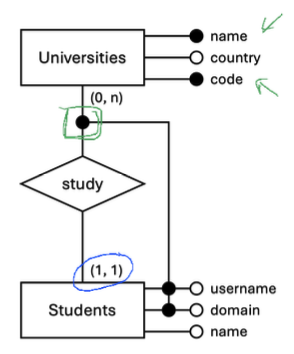
\includegraphics[width=0.85\linewidth, height = 135px]{er5.png} 
    \item Translating ER to Relational Schema:
    \begin{itemize}
      \item \textbf{Rule 1}: Map ER attributes to attributes of relations with meaningful types. (VARCHAR, INTEGER, etc)
      \item \textbf{Rule 2}: Map each entity set to a relation. Candidate keys are mapped to primary keys and UNIQUE NOT NULL.
      \item Composite keys can be specified using table constraints. (PRIMARY KEY (attr1, attr2))
      \item \textbf{Rule 3}: Map each relationship set to a relation. The relation will have the primary keys of the participating entity sets as foreign keys, and any attributes of the relationship set as attributes of the relation. The primary key of the relation will be the combination of the primary keys of the participating entity sets. (PRIMARY KEY (entity1id, entity2id))
      \item Treat aggregates as a relationship set. But its keys can be \textbf{referenced} by other relationship sets.
      \item \textbf{Exception 1}: (0, 1) One-to-many relationship sets can be enforced by removing the keys of the "many" side from the primary key. 
      \item \textbf{Exception 2}: (1, 1) entities in a relationship. Need to enforce minimum cardinality. We merge the entity and the relationship set into a single relation, with the primary key of the entity set as the primary key of the relation.
      \item \textbf{Exception 3}: If partial identification is used, we can merge the weak entity set with the relationship set into a single relation, with the primary key of the dominant entity set and the partial identifier as the primary key of the relation.
    \end{itemize}
  \end{itemize}

  \section{Data Warehousing}

  \begin{itemize}
    \item \textbf{OLTP:} Online Transaction Processing. Focuses on handling a large number of transactions, with a small amount of data per transaction, data up-to-date and consistent, concurrency. (e.g. banking, e-commerce)
    \item \textbf{OLAP:} Online Analytical Processing. Focuses on handling a small number of transactions, with a large amount of data per transaction, static snapshots, query require lots of resources. (e.g. data warehousing, business intelligence)
    \item Kimball's principles for Data Warehousing: Consistency, Accessibility, Security, Adaptability, Acceptance, Decision Support.
    \item \textbf{Dimension Modelling}: A technique for designing data warehouses. It consists of a fact table and dimension tables. The fact table contains the measures (e.g. sales amount, quantity) and foreign keys to the dimension tables. The dimension tables contain the attributes of the dimensions (e.g. product name, customer name).
    \item Each column becomes a dimension.
    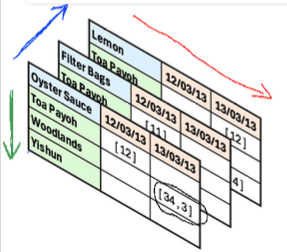
\includegraphics[width=0.77\linewidth, height = 100px]{dim_modelling.png} 
    \item \textbf{Star Schema}: A fact table with multiple dimension tables. The dimension tables are not normalized. (e.g. product dimension table has product name, product category, etc)
    \item \textbf{Fact Table:} Records, for each business process, the measures (aka facts). It also records, for each dimension, the foreign/surrogate key to the dimension table. (e.g. sales fact table has sales amount, quantity, and foreign keys to product, customer, time dimension tables)
    \item Finest available grainularity. Surrogate key is often integers, which are more efficient to join on than natural keys (e.g. product name).
    \item \textbf{Dimension Table:} Records the attributes of the dimensions. It also has a surrogate key as the primary key. (e.g. product dimension table has product, sku, name, category, etc)
    \item Dimension tables can have specialised rows to represent "unknown" or "not applicable" values. Better than \textbf{NULL} values.
    \item Dimension tables are often denormalised, with \textbf{redundant data} and also \textbf{precomputed values}. Improve query performance by reducing the number of joins. 
    \item Hierarchy of dimensions: A dimension can have a hierarchy of attributes. (e.g. time dimension has year, month, day)
    \item \textbf{Snowflake Schema}: A fact table with multiple dimension tables, where the dimension tables are normalized. Avoids data redundancy, but requires more joins.
    \item \textbf{Slice}: Select a layer of the cube by fixing a dimension. WHERE clause.
    \item \textbf{Dice}: Select a subcube by fixing multiple dimensions. WHERE clause.
    \item \textbf{Window functions}: Perform calculations across a set of rows that are related to the current row. (e.g. RANK(), ROW\_NUMBER(), etc)
    \item \textbf{Roll-up}: Aggregate the data by climbing up the hierarchy of a dimension. GROUP BY ROLLUP(B, C, A) equivalent to ordered union of GROUP BY (B, C, A), GROUP BY (B, C), GROUP BY (B), and GROUP BY ().
    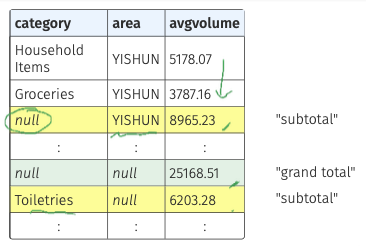
\includegraphics[width=0.85\linewidth, height = 100px]{groupby_cube.png} 
    \item \textbf{Drill-down}: Aggregate the data by climbing down the hierarchy of a dimension. Normal GROUP BY clause.
    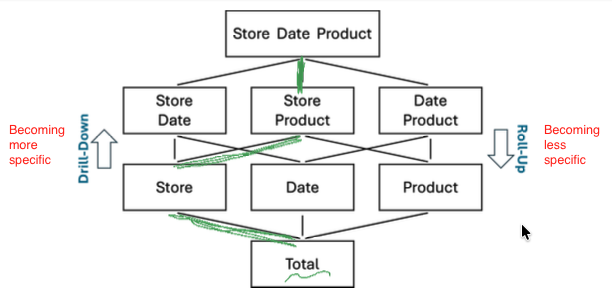
\includegraphics[width=0.85\linewidth, height = 100px]{ru_dd.png} 
    \item \textbf{CUBE}: subclause of GROUP BY that generates all possible combinations of the dimensions. (e.g. GROUP BY CUBE (A,B C) ordered . union of GROUP BY of all combinations of A, B, C). Null values are included.
    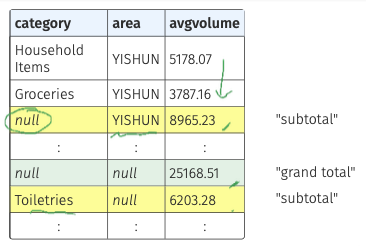
\includegraphics[width=0.85\linewidth, height = 100px]{groupby_cube.png} 
    \item \textbf{Bus Architecture}: A data warehouse architecture where the fact tables and dimension tables are shared across multiple data marts.
    \item Data Integration with ETL $\rightarrow$ dimension modelling for OLAP $\rightarrow$ data optimization $\rightarrow$ OLAP tools.
  \end{itemize}

  \section{Relational Algebra}
  \begin{itemize}
    \item \textbf{Selection} ($\sigma$): Selects rows from a relation that satisfy a given predicate. (e.g. $\sigma_{[age > 30]}(Employees)$). WHERE clause.
    \item \textbf{Projection} ($\pi$): Selects columns from a relation. (e.g. $\pi_{[name, age]}(Employees)$). SELECT clause.
    \item \textbf{Renaming} ($\rho$): Renames a relation or its attributes. (e.g. $\rho(R_1, R_2)$ renames the relation $R_1$ to $R_2$). AS clause.
    \item Example: $\pi[r.attr](\sigma[c](\rho(rel,r)))$
    \item \textbf{Set Operations}: Union ($\cup$), Intersection ($\cap$), Difference ($-$). (e.g. $R \cup S$, $R \cap S$, $R - S$). Requires the relations to be union-compatible (same number of attributes, and corresponding attributes have the same domain).
    \item \textbf{Cross Product} ($\times$): Combines each row of one relation with each row of another relation. (e.g. $R \times S$). Cartesian product. Nested loops join.
    \item Conjunction ($\land$) and Disjunction ($\lor$)
    \item \textbf{Sigma Cascade}: A selection with a conjunction of predicates can be expressed as a cascade of selections. (e.g. $\sigma_{[c_1 \land c_2]}(R)$ equivalent to $\sigma_{[c_1]}(\sigma_{[c_2]}(R))$). Evaluation can be more efficient if the \textbf{inner selection produces fewer rows}.
    \item \textbf{Selection Distributivity over Cross Product}: A selection with a predicate that only involves attributes from one relation can be distributed over the cross product. (e.g. $\sigma_{[c(R)]}(R \times S)$ equivalent to $\sigma_{[c(R)]}(R) \times S$). Evaluation can be more efficient if the selection is applied before the cross product, as it reduces the number of rows in the intermediate result.
    \item \textbf{Selection Distributivity over Union}: A selection with a predicate can be distributed over a union. (e.g. $\sigma_{[c]}(R \cup S)$ equivalent to $\sigma_{[c]}(R) \cup \sigma_{[c]}(S)$). Evaluation can be more efficient if the selection is applied before the union, as it reduces the number of rows in the intermediate result. Same applies to intersection and difference.
    \item \textbf{Pi Cascade}: A projection with a list of attributes can be expressed as a cascade of projections. (e.g. $\pi_{[a_1, a_2]}(R)$ equivalent to $\pi_{[a_1]}(\pi_{[a_1, a_2]}(R))$). Evaluation can be more efficient if the \textbf{inner projection produces fewer columns}.
  \end{itemize}

  \section{Database Tuning}
  \begin{itemize}
    \item PostgreSQL Architecture: SQL Parser and Rewriter $\rightarrow$ Query Planner and Optimizer $\rightarrow$ Executor $\rightarrow$ Memory and Storage Management.
    \item Planner/Optimizer: Generates query plans using catalogue and statistics, choose plan with least estimated cost.
    \item Cost is estimated based on the number of rows processed, the number of disk I/O operations, and the CPU time required for the operations.
    \item Execution Plan: DAG/Tree of operations. 
    \item Types: Sequential Scan, Index Scan, Bitmap Index Scan, Bitmap Heap Scan, Nested Loop Join, Hash Join, Merge Join, Aggregate Operation etc.
    \item Total query time: query planning time + execution time, network latency, client overhead.
    \item \textbf{EXPLAIN (ANALYZE, VERBOSE)} command: shows the execution plan, execution time, row count for each step. (e.g. EXPLAIN ANALYZE SELECT * FROM Employees WHERE age $>$ 30)
    \item Only supports: SELECT, INSERT, UPDATE, DELETE, EXECUTE, CREATE TABLE, DECLARE.
    \item In the query plan: (cost=startup cost..total cost rows=estimated rows width=estimated row width (in bytes)). Startup cost is the cost before the first row is returned, total cost is cost of executing the node (including its children).
    \item \textbf{pg\_tables}: Catalog table that contains information about tables in the database. (e.g. SELECT * FROM pg\_tables)
    \item \textbf{pg\_indexes}: Catalog table that contains information about indexes in the database. (e.g. SELECT * FROM pg\_indexes)
    \item \textbf{pg\_stats/pg\_statistics}: Catalog table that contains statistics about the distribution of values in the columns of the tables. Populated by the ANALYZE command (e.g. SELECT * FROM pg\_stats)
    \item \textbf{pg\_attributes}: Catalog table that contains information about the attributes (columns) of the tables. (e.g. SELECT * FROM pg\_attributes)
    \item \textbf{Total time of a node} = product of actual time * loops
    \item \textbf{VACUUM}: Reclaims storage occupied by dead tuples. Also updates statistics for the query planner. (e.g. VACUUM ANALYZE Employees)
    \item \textbf{Index Types}: B-tree (default, supports equality and range queries), Hash (supports equality queries), GIN (supports full-text search), GiST (supports spatial data), BRIN (supports large tables with natural ordering).
    \item \textbf{Indexes} generally slow down write operations (INSERT, UPDATE, DELETE) because the index also needs to be updated. However, they can significantly speed up read operations (SELECT) by allowing the query planner to quickly locate the relevant rows.
    \item \textbf{PostgreSQL} automatically creates \textbf{B-tree unique indexes for primary key and unique constraints}. However, it does not automatically create indexes for foreign keys.
    \item \textbf{SYNTAX}: CREATE INDEX index\_name ON table\_name (column\_name...);
    \item We can create unique indexes. CREATE UNIQUE INDEX...
    \item We can use WHERE to create partial indexes.
    \item \textbf{Clustering}: Reorganizes the physical storage of the table to match the order of an index. This can improve the performance of queries that use the index. (e.g. CLUSTER Employees USING idx\_age)
    \item \textbf{A table can only be clustered on one index at a time.} Clustering needs to be \textbf{reapplied} after any write operation that modifies the clustered index.
    \item \textbf{Multi-column Indexes}: The order of the columns in the index matters. Index is used if condition involves \textbf{prefix} of the multi-column index (e.g. CREATE INDEX idx\_age\_name ON Employees (age, name))
   \end{itemize}

  \subsubsection*{Data Retrieval Operations}
  \begin{itemize}
    \item \textbf{Sequential Scan}: Reads the entire table sequentially. Used when there is no index, or when the query planner estimates that it will be faster than using an index (e.g. when a large portion of the table is being scanned).
    \item \textbf{Sort}: Sorts the rows based on the specified columns. Used for ORDER BY, GROUP BY, DISTINCT, etc. (Quick Sort, Merge Sort, etc)
    \item \textbf{Grouping/Aggregation}: Groups the rows based on the specified columns and applies aggregate functions (e.g. SUM, COUNT, AVG) to each group. Used for GROUP BY, aggregate functions without GROUP BY, etc.
    \item \textbf{Unique}: Removes duplicate rows from the result set. Used for DISTINCT, etc. \textbf{Note:} Don't use DISTINCT for candidate key columns.
    \item \textbf{Index Only Scan}: Uses an index to retrieve the values of the indexed columns, without accessing the table. Used when index is a covering index.
    \item \textbf{Index Scan}: Uses an index to retrieve the values of the indexed columns, and then accesses the table to retrieve the values of the non-indexed columns. Used when there is an index on the columns used in the WHERE clause, but the index is not a covering index.
    \item \textbf{Bitmap Heap Scan}: Uses a bitmap index scan to retrieve the row locations of the matching rows, and then accesses the table to retrieve the values of the columns. Used when there is an index on the columns used in the WHERE clause, but the index is not a covering index, and the query planner estimates that it will be faster than using an index scan (e.g. when a large portion of the table is being scanned).
    \item \textbf{Bitmap Index Scan}: Uses a bitmap index to retrieve the row locations of the matching rows. Can be used for conjunctions or disjunctions of predicates on indexed columns.
  \end{itemize}

  \section{PostgreSQL Cheatsheet}
  \begin{itemize}
    \item \textbf{Syntax overview}: SQL is case-insensitive; statements end with `;`. Keywords: SELECT, INSERT, UPDATE, DELETE, CREATE, ALTER, DROP, GRANT, REVOKE.
    \item \textbf{Common options}: `EXPLAIN`/`EXPLAIN ANALYZE`, `SET` to change runtime parameters, `BEGIN`/`COMMIT`/`ROLLBACK` for transactions, `VACUUM`, `ANALYZE`, `CREATE INDEX CONCURRENTLY`.
    \item \textbf{Comparison qualifiers}: `$>$ ALL`, `$<$ ALL`, `$>=$ ANY`, `SOME` synonyms; compare against every/any value from subquery. `IS NULL`/`IS NOT NULL` for null tests.
    \item \textbf{Pattern matching}: `LIKE` (case‑sensitive), `ILIKE` (case‑insensitive); `\%` = any string, `\_` = single char. Use POSIX regex `~`/`~*`/`!~`/`!~*`.
    \item \textbf{Existence}: `EXISTS (subq)` returns true if subquery yields rows; `NOT EXISTS` negates. Often correlated with outer query.
    \item \textbf{Membership}: `expr IN (a,b,...)` or `IN (subquery)`; `NOT IN` negates but beware NULLs (use `NOT EXISTS` if null-safe).
    \item \textbf{For‑all logic}: express `for every` via double `NOT EXISTS` (or use `ALL`/`$>=$ ALL` where applicable). e.g.
      `WHERE NOT EXISTS (SELECT 1 FROM t1 x WHERE NOT EXISTS (SELECT 1 FROM t2 y WHERE y.key=x.key AND ...))`.
      Alternates: anti-join pattern `LEFT JOIN … WHERE b.id IS NULL`.
    \item \textbf{Set operations}: UNION (remove duplicates), UNION ALL, INTERSECT, EXCEPT. All arms must have same column count and compatible types; order and column names come from first query.
    \item \textbf{COALESCE}: Returns the first non-null value in the list. (e.g. COALESCE(column1, column2, 'default')) (e.g. AVG(COALESCE(l.rd\_date-l.bd\_date, CURRENT\_DATE - bd\_date), 2) AS average)
    \item For MAX queries with potentially multiple rows with the same maximum value, we can use a subquery to find the maximum value, and then join it back to the original table to retrieve all rows with that maximum value. (e.g. SELECT name FROM Employees WHERE age = (SELECT MAX(age) FROM Employees))
    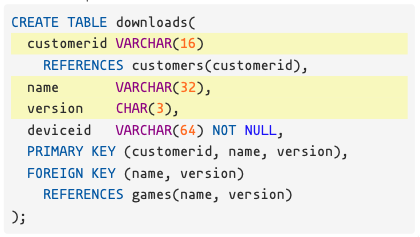
\includegraphics[width=0.85\linewidth, height = 100px]{sql_create_table.png} 
  \end{itemize}


\end{multicols*}

\end{document}
